\documentclass[12pt]{article}

\usepackage[utf8]{inputenc}
\usepackage{amsmath}
\usepackage{graphicx}
\usepackage{titlesec}
\usepackage{tcolorbox}
\usepackage{titling}
\usepackage{circuitikz}
\usepackage{enumitem}
\usepackage{wrapfig}
\usepackage{float}
\usepackage{pgfplots}
\usepackage{hyperref}
\usepackage{tikz}
\usetikzlibrary{patterns}
\pgfplotsset{compat=1.18}

\title{\bfseries Laborator Electricitate 4}
\author{Sîrghe Matei}
\date{\today}

\titleformat{\section}
  {\normalfont\Large\bfseries}{\thesection}{1em}{}

\begin{document}

\maketitle

\section{Problemă}
O cantitate de sarcină Q este distribuită sub formă de strat subțire sferic a=raza sferei. De-a lungul unui diametr al acestei sfere, se plimbă un corp punctiform cu sarcină q.Calculați forța cu care acționează sarcina Q asupra corpului punctiform cu sarcina q.

\subsection{Explicații Matematică}

\begin{figure}[H]
    \centering
    \noindent
    \begin{minipage}{0.45\textwidth}
        \centering
        \begin{tikzpicture}[scale=0.75]
            \draw (0,0) circle (2cm);
            \draw (0,0) ellipse (2cm and 1cm);
            \draw[->] (-2,-2) -- (2,2) node[right] {$\vec{z}$};
            \draw[->] (-4,0) -- (4,0) node[right] {$\vec{x}$};
            \draw[->] (0,-4) -- (0,4) node[right] {$\vec{y}$};
        \end{tikzpicture}
        \caption{Cerc, elipsă și vectori}
        \label{fig:circle_ellipse_vectors}
    \end{minipage}
    \hfill
    \begin{minipage}{0.45\textwidth}
        \centering
        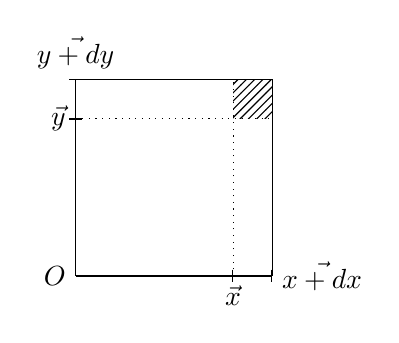
\begin{tikzpicture}
            \draw[-] (0,0) -- (0,0)node[anchor=east] {$O$};
            \draw[-|] (0,0) -- (2,0) node[anchor=north] {$\vec{x}$};
            \draw[-|] (2,0) -- (2.5,0) node[anchor=west] {$\vec{x+dx}$};
            \draw[-|] (0,0) -- (0,2) node[anchor=east] {$\vec{y}$};
            \draw[-|] (0,2) -- (0,2.5) node[anchor=south] {$\vec{y+dy}$};

            \fill[pattern=north east lines] (2,2) rectangle (2.5,2.5);
            \draw[dotted] (0,2) -- (2.5,2) {};
            \draw[dotted] (2,0) -- (2,2.5) {};
            \draw[-] (0,2.5) -- (2.5,2.5) {};
            \draw[-] (2.5,0) -- (2.5,2.5) {};
        \end{tikzpicture}
        \caption{Coordonate Carteziene}
        \label{fig:vectors_in_plane}
    \end{minipage}
\end{figure}

\begin{figure}[H]
    \centering
    \noindent
    \begin{minipage}{0.45\textwidth}
        \centering
        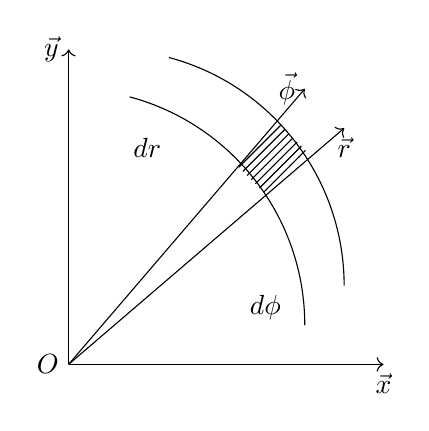
\begin{tikzpicture}
            \draw[-] (0,0) -- (0,0)node[anchor=east] {$O$};
            \draw[->] (0,0) -- (4,0) node[anchor=north] {$\vec{x}$};
            \draw[->] (0,0) -- (0,4) node[anchor=east] {$\vec{y}$};
            \draw (3,0.5) arc[start angle=0, end angle=75, radius=3cm];
            \draw (3.5,1) arc[start angle=0, end angle=75, radius=3cm];

            \draw[->] (0,0) -- (3.5,3) node[anchor=north] {$\vec{r}$};
            \draw[->] (0,0) -- (3,3.5) node[anchor=east] {$\vec{\phi}$};

            \draw (2.5,1) node[anchor=north] {$d\phi$};
            \draw (1,3) node[anchor=north] {$dr$};

            \fill[pattern=north east lines, rotate=45] (3.30,-0.25) rectangle (4.05,0.25);
        \end{tikzpicture}
        \caption{Coordonate Polare}
        \label{fig:vectors_in_plane}
    \end{minipage}
    \hfill
    \begin{minipage}{0.45\textwidth}
        \centering
        \begin{tikzpicture}[scale=0.75]
            \draw (0,0) circle (2cm);
            \draw (0,0) ellipse (2cm and 1cm);
            \draw[->] (-2,-2) -- (2,2) node[right] {$\vec{z}$};
            \draw[->] (-4,0) -- (4,0) node[right] {$\vec{x}$};
            \draw[->] (0,-4) -- (0,4) node[right] {$\vec{y}$};
        \end{tikzpicture}
        \caption{Sfera electrizată}
        \label{fig:circle_ellipse_vectors}
    \end{minipage}
\end{figure}

\end{document}